\documentclass[xetex, xcolor=dvipsnames]{beamer}
\usepackage{animate}
\usepackage{style}
\usepackage{../symbols}
\mode<presentation>

% \institute{Дальневосточный Федеральный Университет}
\title{
	Численный анализ диффузионных моделей распространения вирусов 
}
\subtitle{}
\author{
	Максимов П.А. \\ \vspace{10pt}
	Научный руководитель: \\ к.ф.-м.н. Бризицкий Р.В., д.ф.-м.н. Алексеев Г.В.
}
\date{Владивосток, 2022}

\begin{document}
	
	\begin{noheadline}
		\frame {
			\fefuheader
			\titlepage
		}
	\end{noheadline}
	
	\frame {
		\frametitle{Цели}

		\begin{enumerate}
			\item Рассмотреть модели распространения вирусов
			\item Провести численные эксперименты одномерной и двумерной моделей
			\item Поставить стационарную краевую задачу для диффузионной модели распространения
			\item Оценить оптимальные решения поставленной задачи
		\end{enumerate}
	}

	\frame {
		\frametitle{Примеры моделей}
		\begin{enumerate}
			\item Модель SIR:
			\[ \begin{cases} 
				\displaystyle \dpart{S}{t} &= - \kappa S I - D S \Delta I, \\ 
				\displaystyle \dpart{I}{t} &= \kappa S I + D S \Delta I - \dfrac{1}{\tau} I, \\
				\displaystyle \dpart{R}{t} &= \dfrac{1}{\tau} I,
			\end{cases} \]
			с начально-краевыми условиями:
			\[ \begin{cases} 
				S\ont_{t_0} &= S_0(\mathbf{x}), ~ S\ont_{\Gamma} = S_{\Gamma}(t, \mathbf{x}), \\
				I\ont_{t_0} &= I_0(\mathbf{x}), ~ I\ont_{\Gamma} = I_{\Gamma}(t, \mathbf{x}), \\
				R\ont_{t_0} &= R_0(\mathbf{x}), ~ R\ont_{\Gamma} = R_{\Gamma}(t, \mathbf{x}).
			\end{cases} \]
			Переход между состояниями происходит по закону
			\[ S \xrightarrow{\kappa} I \xrightarrow{\frac{1}{\tau}} R, \]
			и система удовлетворяет закону сохранения:
			\[ \dpart{S}{t} + \dpart{I}{t} + \dpart{R}{t} = 0 \]

		\end{enumerate}
	}

	\frame{

		\frametitle{Численный эксперимент для одномерной модели SIR}

		%Параметры статьи Постникова
		\begin{figure}
			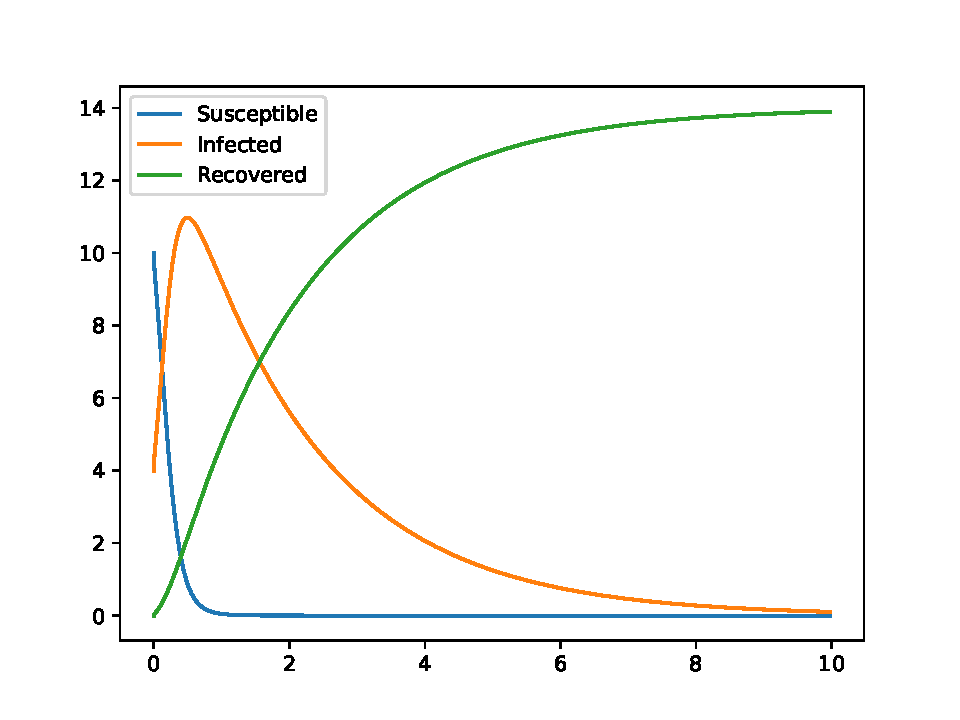
\includegraphics[width=0.7\textwidth]{../additional/1dimsir.pdf}
			\caption{Решение при параметрах $\kappa = 0,55$, $\tau = 2$, $S_0 = 10$, $I_0 = 4$, $R_0 = 0$}
		\end{figure}
		
		%Временной диапазон не фиксирован, график показывает поведение подверженных заболеванию, инфицированных и вылечивающихся
	}

	\frame{
		\frametitle{Численный эксперимент двумерной диффузионной модели SIR}

		\begin{figure}
			\animategraphics[width=0.7\textwidth]{9}{plots/fem/plot_0_}{1}{9}
			\caption{Распределение инфицированных особей в двумерном пространстве при параметрах $\kappa = 0,55$, $\tau = 2$}
		\end{figure}
	}

	\frame{
		\frametitle{Постановка краевой задачи}

		Рассмотренные диффузионные модели в общем случае являются нелинейными. Поставим краевую задачу, которая позволит обобщить такие модели. Рассмотрим стационарный случай для нелиейного уравнения реакции--диффузии--конвекции, рассматриваемого ограниченной области $\Omega \subset \R^3$
		\begin{equation}
			\label{4a}
				- \div{(\lambda(\mathbf{x}) \grad{\vp})} 
				+ \mathbf{u} \cdot \grad{\vp}
				+ k (\vp, \mathbf{x}) \vp 
				= f \text{ в } \Omega, 
		\end{equation}
		Предполагается, что  граница $\Gamma$ области $\Omega$ состоит из двух частей $\Gamma_D$ и $\Gamma_N$ и уравнение (\ref{4a}) рассматривается при смешанных краевых условиях:
		\begin{equation}
			\label{4}
				\vp = \psi \text{ на } \Gamma_D, ~
				\lambda (\mathbf{x}) 
				\left( \partial \vp / \partial n + \alpha(\vp, \mathbf{x})\vp \right)
				=\chi \text{ на } \Gamma_N.
		\end{equation}
	}

	\frame{
		\frametitle{Функциональные пространства}

		Введем следующие функциональные пространства:
		\[
			L_{+}^{p} (D) = \braces{
				k \in L^p (D): k \ge 0 
			}, ~ p \ge 3/2, 
		\] 
		\[ 
			Z = \braces{ 
				\mathbf{v} \in L^4 (\Omega)^3: 
				\div{\mathbf{v}} = 0 \text{ в } \Omega, 
				~ \mathbf{v \cdot n}\ont_{\Gamma_N} = 0 
			},
		\] 
		\[ 
			H^{s}_{\lambda_0} (\Omega) = \braces{ 
				h \in H^{s} (\Omega): h \ge \lambda_0 > 0 \text{ в } \Omega 
			}, s > 3/2, 
		\] 
		\[ 
			\cT= \braces{ 
				\vp \in H^1 (\Omega): \vp \ont_{\Gamma_D} = 0 
			}.
		\]
	}
	
	\frame{

		Будем предполагать, что нелинейности $k \pares{\vp,\cdot} \vp$ и $\alpha \pares{\vp, \cdot} \vp$ являются монотонными в следующим смысле:
		\begin{enumerate}
			\item \label{rconds5}
				$\pares{ k (\vp_1, \cdot) \vp_1 - k (\vp_2, \cdot) \vp_2, \vp_1 - \vp_2} \ge 0$ $\forall \vp_1, \vp_2 \in H^1 (\Omega)$;

			\item \label{rconds6}
				$ \pares{ \alpha (\vp_1, \cdot) \varphi_1 - \alpha (\vp_2, \cdot) \vp_2, \vp_1 - \vp_2}_{\Gamma_N} \ge 0$ $\forall \vp_1, \vp_2 \in H^1 (\Omega)$.

		\end{enumerate}

		Пусть так же функции $ k (\vp, \cdot) $ и $\alpha (\vp, \cdot)$ ограничены в том смысле, что $\forall A_1(k), B_1(k) > 0$, и $\forall A_2(\alpha), B_2(\alpha) > 0$, такие, что
		\begin{enumerate}
			\setcounter{enumi}{2}

			\item \label{rconds7}
				$\norm{ k (\vp, \cdot) }_{L^p (\Omega)} \le A_1 \norm{\vp}_{1,\Omega}^r + B_1$ $\forall \vp \in H^1 (\Omega)$ при $p \ge 3/2$, $r \ge 0$ ;

			\item \label{rconds8}
				$\norm{\alpha (\vp, \cdot)}_{L^q (\Gamma_N)} \le A_2 \norm{\vp}_{1,\Omega}^l + B_2$ $\forall \vp \in H^1 (\Omega)$ при $q \ge 2$, $l \ge 0$.

		\end{enumerate}
	}

	\frame{

		\frametitle{Мультипликативная задача управления}

		Пусть функция $k(\vp, \mathbf{x})$ удовлетворяет условию
		\begin{enumerate}
			\setcounter{enumi}{4}
			\item \label{rconds9}
				$k(\vp, \mathbf{x}) = \beta (\mathbf{x}) k_0 (\vp)$, где $\beta (\mathbf{x}) \in H^1_+ (\Omega)$, $k_0 (\vp) \in L^2_+ (\Omega)$ для всех $\vp \in H^1 (\Omega)$, удовлетворяет свойству (\ref{rconds7}) при $p>2$ и в любом шаре $B_r = \braces{ \vp \in H^1 (\Omega): \norm{\vp}_{1,\Omega} \le r }$ радиуса $r$ справедливо неравенство:
				\begin{equation}
					\label{x_eq}
					\norm{k_0 (\vp_1) - k_0 (\vp_2) }_{\Omega} 
					\le L_3 \norm{\vp_1 - \vp_2}_{L^4 (\Omega)} 
					\quad \forall \vp_1, \vp_2 \in B_r.
				\end{equation}
		\end{enumerate}

		Введем пространство $Y ={\cT}^{*} \times H^{1/2} (\Gamma_D)$, положим $u = (\lambda, \beta)$, $K= K_1 \times K_2$ и введем оператор $ F = (F_1, F_2): H^1 (\Omega) \times K \to Y $ по формулам:
		\[
			\begin{split}
				\vprod{F_1 (\vp, u), h} &= 
				\pares{\lambda \grad{\vp}, \grad{h}} + \pares{\beta (\mathbf{x}) k_0 (\vp) \vp, h} +
				\pares{\mathbf{u} \cdot \grad{\vp}, h} + \\
				&+ \pares{\lambda \alpha (\vp, \mathbf{x}) \vp, h}_{\Gamma_N} -
				\pares{f, h} - \pares{\chi, h}_{\Gamma_N},
			\end{split}
		\]
		\[
			F_2 (\vp) = \vp\ont_{\Gamma_D} - \psi,
		\]
		и перепишем в виде $F(\vp, u) = 0$.
	}

	\frame{

		Рассматривая это равенство как условное ограничение на состояние $\vp \in H^1 (\Omega)$ и управление $u \in K$, получим задачу условной минимизации:
		\begin{equation}
			\label{3.1}
			\begin{split}
				J \pares{\vp, u} &\equiv \frac{\mu_0}{2} I \pares{\vp} 
				+ \frac{\mu_1}{2} \norm{\lambda}^2_{s,\Omega} 
				+ \frac{\mu_2}{2} \norm{\beta}^2_{1,\Omega} \rightarrow \inf, ~ \\
				F \pares{\vp, u} &= 0, ~ \pares{\vp, u} \in H^1 (\Omega) \times K.
			\end{split}
		\end{equation}
		Здесь $I: H^1 (\Omega) \to \R$. %-- функционал, полунепрерывный снизу относительно слабой сходимости.

		Будем использовать следующие функционалы качества: 
		\begin{equation}
			\label{cost_f}
			I_1 (\vp) = \norm{\vp - \vp^d}^2_Q = 
			\int_Q \abs{\vp - \vp^d}^2 d \mathbf{x}, \quad 
			I_2 (\vp) = \norm{\vp - \vp^d}_{1,Q}^2.
		\end{equation}

		Из изложенного ранее, получим следующую оценку:
		\begin{equation}
			\label{cbeta}
			\norm{\lambda}_{s,\Omega} \le C_\lambda ~ \forall \lambda \in K_1, ~
			\norm{\beta}_{1,\Omega} \le C_\beta ~ \forall \beta \in K_2, 
		\end{equation}
		где $C_\lambda, C_\beta > 0$. 

	}

	\frame{

		\frametitle{Вывод системы оптимальности}

		% Следуя общей теории гладко-выпуклых экстремальных задач
		Введем элемент $\mathbf{y}^{*} = \pares{\theta, \zeta} \in Y^{*}$, на который будем ссылаться как на сопряженное состояние, и введем Лагранжиан $\Lg: H^1 (\Omega) \times K \times Y^{*} \to \R$ по формуле
		\begin{equation}
			\label{Lagran}
			\begin{split}
				\Lg(\vp, u, \mathbf{y}^{*}) &= J(\vp, u) 
				+ \vprod{\mathbf{y}^{*}, F(\vp, u)}_{Y^{*} \times Y} 
				\equiv J(\vp, u) 
				+ \vprod{F_1(\vp, u), \theta}_{\cT^{*} \times \cT} + \\
				&+ \vprod{\zeta, F_2(\vp, u)}_{\Gamma_D},
			\end{split}
		\end{equation}

		На основе анализа системы оптимальности для конкретного коэффициента реакции 
		$k(\vp, \mathbf{x}) = 
			\beta_0 (\mathbf{x}) k_0 (\vp) \equiv 
			\beta_0 (\mathbf{x}) \vp^2
		$ и коэффициента массобмена $\alpha (\vp) = \abs{\vp}$, а также для конкрентных функционалов качества будут получены оценки локальной устойчивости оптимальных решений.

	}

	\frame{

		Из теоремы Лакса-Мильграма вытекает, что для любых $f \in L^2 (\Omega)$ и $\psi \in H^{1/2} (\Gamma_D)$ существует единственное решение $\tau \in H^1 (\Omega)$ линейной задачи 
		\begin{equation}
			\label{LinPr}
			\pares{\hat \lambda \grad{\tau}, \grad{h}} 
			+ 3 \pares{\hat \beta \hat \vp \tau, h} 
			+ \pares{\hat \lambda \abs{\hat \vp} \tau, h}_{\Gamma_N} 
			+ \pares{\mathbf{u} \cdot \grad{\tau}, h} = \pares{f, h} ~ \forall h \in \cT,
		\end{equation}
		\[ \tau\ont_{\Gamma_D} = \psi. \]

	}

	\frame{

		\frametitle{Оценки локальной устойчивости оптимальных решений}

		% Установим достаточные условия единственности и устойчивости решений конкретных экстремальных задач. 
		Проведем анализ следующей экстремальной задачи, отвечающей функционалу качества $I_1 (\vp) = \norm{\vp - \vp^d}^2_Q$:
		\begin{equation}
			\label{func1}
			\begin{split}
				J(\vp, u) &= \frac{\mu_0}{2} I_1 (\vp) 
				+ \frac{\mu_1}{2} \norm{\lambda}^2_{s,\Omega} 
				+ \frac{\mu_2}{2} \norm{\beta}^2_{1,\Omega} \to \inf, \\
				F(\vp, u, f) &= 0, ~ \pares{\vp, u} \in H^1 (\Omega) \times K.
			\end{split}
		\end{equation} 
		Обозначим через $\pares{\vp_1, u_1}$ решение задачи (\ref{func1}), отвечающее заданным функциям $\vp^d= \vp^d_1 \in L^2(Q)$ и $f = f_1 \in L^2 (\Omega)$. 

		Через $\pares{\vp_2, u_2}$ обозначим решение задачи (\ref{func1}), отвечающее возмущенным функциям $\tilde \vp^d = \vp^d_2 \in L^2(Q)$ и $\tilde f = f_2 \in L^2 (\Omega)$. Полагая $\vp^d = \vp^d_1 - \vp^d_2$, получим
		\begin{equation}
			\label{func3}
			\begin{split}
				\vprod{I_1' (\vp_i), \tau} &= 2 \pares{\vp_i - \vp^{d}_i, \tau}_Q, \\
				\vprod{I_1' (\vp_1) - \tilde I_1' (\vp_2), \tau} &= 2 \pares{ \pares{\vp, \tau}_Q - \pares{\vp^d, \tau}_Q }, ~ i=1, 2.  
			\end{split}
		\end{equation}

	}

	\frame{

		Для множителей Лагранжа $\theta_i \in {\cT}$, отвечающие решениям $(\vp_i, u_i)$,  принимают вид
		\begin{equation}
			\label{theta3}
			\begin{split}
				\pares{\lambda_i \grad{\tau}, \grad{\theta_i}} 
				&+ 3 \pares{\beta_i \vp^2_i \tau, \theta_i} 
				+ 2 \pares{\lambda_i \abs{\vp_i} \tau, \theta_i} 
				+ \pares{\mathbf{u} \cdot \grad{\tau}, \theta_i} + \\
				&+ \vprod{\zeta_i, \tau}_{\Gamma_D} =
				- \mu_0 \pares{\vp_i - \vp^d_i, \tau}_Q \quad 
				\forall \tau \in H^1 (\Omega), ~ i=1, 2.
			\end{split}
		\end{equation}

	}

	\frame{

		\frametitle{Результаты}

		Из проведенных рассчетов, получим следующие оценки:
		\[
			\begin{split}
				&\norm{\lambda}_{s,\Omega} 
				\le 
					\sqrt{\mu_0 / \varepsilon_1 \mu_1} ~
					\pares{
						\omega_3 
						\norm{f}_\Omega 
						+ \pares{\omega_4 + 0.5} 
						\norm{\vp^d}_Q
					}, \\
				&\norm{\beta}_{1,\Omega} 
				\le 
					\sqrt{\mu_0 / \varepsilon_2 \mu_2} ~ 
					\pares{
						\omega_3 
						\norm{f}_\Omega 
						+ \pares{\omega_4 + 0.5} 
						\norm{\vp^d}_Q
					},
			\end{split}
		\]
		из чего вытекает оценка для разности решений $\vp_1 - \vp_2$:
		\begin{equation}
			\label{est12}
			\begin{split}
				\norm{\vp_1 - \vp_2}_{1, \Omega} 
				&\le  
					C_{*} 
					\pares{
						a \omega_3 
						\sqrt{\mu_0 / \varepsilon_1 \mu_1} 
						+ b \omega_3 
						\sqrt{\mu_0 / \varepsilon_1 \mu_1} 
						+ 1
					} \\
					&\norm{f_1- f_2}_\Omega + \\
				& + C_{*} 
					\pares{\omega_4 + 0.5} 
					\pares{
						a \omega_3 
						\sqrt{\mu_0 / \varepsilon_1 \mu_1} 
						+ b \omega_3 
						\sqrt{\mu_0 / \varepsilon_1 \mu_1}
					} \\
					&\norm{\vp^d_1 - \vp^d_2}_Q. 
			\end{split}
		\end{equation} 

		%Стоит отметить, что ...
	}

	\frame{

		\frametitle{Заключение}
		На основе проведенного анализа, можно сделать вывод об устойчивости численных алгоритмов решения прямых и обратных задач для нелинейных стационарных диффузионных моделей при определенных коэффициентах и параметрах.

	}

\end{document}
